%================================================================================
%=============================== DOCUMENT SETUP =================================
%================================================================================

%\documentclass[lang=ngerman,inputenc=utf8,fontsize=10pt]{ldvarticle}
\documentclass[lang=ngerman,inputenc=utf8,fontsize=10pt]{ldvarticle}
%PACKAGES

\usepackage{parskip}
\usepackage{subfigure}
\usepackage{ifthen}
\usepackage{comment}
\usepackage{color}
\usepackage{colortbl}
\usepackage{soul}
\usepackage{tikz}
\usetikzlibrary{shapes,arrows}
\usepackage{tabularx}
\usepackage{lipsum}
\usepackage{pgfgantt}
\usepackage{amsmath}

\usepackage{color}

\usepackage[backend=biber,style=ieee,
doi=false,isbn=false,url=false,eprint=false]{biblatex}
\addbibresource{Relevant.bib}

\definecolor{lightgray}{rgb}{0.75,0.75,0.75}


\usepackage{tikz}
\usetikzlibrary{calc}
\usetikzlibrary{calendar}

\newcommand{\countweek}{\ifdate{equals=01-01}{\setcounter{weekcounter}{0}}{} \ifdate{Thursday}{\stepcounter{weekcounter}}{}}

% GanttHeader setups some parameters for the rest of the diagram
% #1 startdate
% #2 enddate
% #3 with of 
\def\GanttHeader#1#2#3{%
\newcounter{weeks}
\newcounter{weekcounter}
\def\withdes{3cm}
\def\hrows{0.4cm}
%get number of weeks
\calendar [dates=#1 to #2,day code={},
execute after day scope=
{\ifdate{Thursday}{\stepcounter{weeks}}{}}];

%get the currend KW
\calendar [dates=2021-01-01 to #1+-1,day code={},
execute after day scope=
{\countweek}];

%calcualate the shifts
\pgfmathsetmacro{\dayshift}{(\textwidth-\withdes)/(\theweeks*7)}

\tikzstyle{every day}=[anchor=mid]
\calendar [dates=#1 to #2,day code={},
execute after day scope=
{\countweek \ifdate{Thursday}{\node {\tiny\textbf{\theweekcounter}};}{} 
	\ifdate{Sunday}{\draw[thick] (0,-0.5*\hrows) -- +(0,\hrows);}{} 
	\ifdate{day of month=15}{\node[] at (0,\hrows) {\small{\tikzmonthtext}};}{} 
	\ifdate{day of month=1}{\draw[thick] (0,0.5*\hrows) -- +(0,\hrows);}{}
	\pgftransformxshift{\dayshift}}] 
at (\withdes,0); %set position

%setup descriptions
\draw[very thick] (0,0.5*\hrows) rectangle +(\withdes, \hrows);
\draw[very thick] (0,-0.5*\hrows) rectangle +(\withdes, \hrows);
\draw[very thick] (\withdes,0.5*\hrows) rectangle +(\textwidth-\withdes, \hrows);
\draw[very thick] (\withdes,-0.5*\hrows) rectangle +(\textwidth-\withdes, \hrows);
\node[] at (0.5*\withdes,\hrows) {\small{\textbf{Month}}};
\node[] at (0.5*\withdes,0) {\small{\textbf{Week}}};
}


% This macro adds a task to the diagram
% #1 Row of the Task
% #2 Task's name
% #3 Starting Week
% #4 Duration (Weeks)
\def\Task#1#2#3#4{%
\begin{scope}[shift={(0,-0.2*\hrows-#1*\hrows)}]
  \filldraw[fill=black!20,thick] (0,-0.5*\hrows) rectangle +(\textwidth, \hrows);
\node[anchor=west] at (1mm,0) {\small{\textbf{#2}}};
 \filldraw[color=red] (\dayshift*7*#3+\withdes,-0.45*\hrows) rectangle +(\dayshift*7*#4+0cm,0.9*\hrows);
  \foreach \x in {0,...,\theweeks} {
    \draw[thick] (\dayshift*7*\x+\withdes,-0.5*\hrows) -- +(0,\hrows);
}
\end{scope}
}







\DeclareMathOperator{\vect}{vec}

%================================================================================
%================================= TITLE PAGE ===================================
%================================================================================

\title{Matrix representation as sum of local low rank matricies}
\subtitle{Projectplan}
\author{Stepahn Nüßlein}

\date{\today}

\begin{document}


	\maketitle
	\thispagestyle{empty}
	\vspace*{2cm}
	\hrule

\section*{Motivation}

\begin{itemize}
	\item Matrices for fully connected Layers get larger -> Computational expensive 
	\item Matrix approximations with reduced computational cost
	\item Both approxiamtion of Matrix in some Norm important ($\|\|_F$,$\|\|_1$,$\|\|_\infty$ or similar) also Accuracy on Data set
\end{itemize}




\vspace*{1cm}
\hrule

\newpage

\section{Project Description}

\subsection*{Goals}

\begin{itemize}
	\item Find Matrix approximation with reduced cost
	\item Get some theoretical predictions on the behavior
	\item Find algorithm to construct said approximation
	\item Evaluate approximation in practical examples
\end{itemize}











\subsection*{Approach}

These assumptions and properties are underlying the idea:
\begin{itemize}
	\item Matrices in Fully connected layers often have full rank -> so no rank reduction easily possible (with some caveats, as it is not certain that this is the relevant ingredient) \cite{martin_implicit_2018}
	\item The order of inputs/outputs is not important $A$ is equivalent to $\Pi_o A \Pi_i$ with $\Pi_i$ and $\Pi_o$ permutation matrices as the ordering of the neurons can be changed. 
	\item To get the optimal trade of between accuracy and cost it should be possible to set them at a late stage in the algorithm
\end{itemize}

Approximate the given Matrix $A \in \mathbb{R}^{n \times m}$ using the representation

\begin{equation}\label{key}
A = \sum_{i=1}^{k} a_i u_i v_i^\top 
\end{equation}

With $k$ not necessarily $\leq \min(n,m)$ and most of $u_i$ and $v_i$ sparse. Without loss of generality we can assume $a_i \geq 0$. The $a_i$ are ordered in decreasing order.
Therefore the vectors $u_i$ and $v_i$ have some constraint on their norm. 
Also sparsity has to be defined in a more rigid way.

The expression can be viewed as a modification of the SVD.
Alternatively the weighted sum can be expressed as a Matrix-vector product.
\begin{equation}\label{eq:vec}
\vect(A) = \sum_{i=1}^{k} a_i\vect(u_i v_i^\top) = \left[\vect(u_1 v_1^\top), \cdots, \vect(u_k v_k^\top)\right] a = \left[v_1 \otimes u_1, \cdots, v_k\otimes u_k\right] a
\end{equation}

It is possible to express different matrix structures with the proposed representation.
Hirarchical matricies can be converted trivially. Sequentially semiseperable and semiseperable are technically possible.
Also said structures with row and/or collumn permutations and sum of said are possible.

[Note: Additional further ideas: Maybe transformation in $P_1 T_{[A,B,C,D]} P_2$ where the $P$s are (sub)permutations and the $T$ is a state Space Model]

Unlike the hierarchical matrices the low rank structures are overlapping. 
This poses the risk that it might be ill defined and the prone to numerical errors. Compare it to \eqref{eq:vec}. The vectors might be linearly dependent. 
%Risiko mathematisch -> bei vielen anderen Strukturen (besonders hirarchischen) gibt es keine Überlappungen, hier aber schon damit Risiko dass numerische Probleme auftauchen.
Therefore it might be worthwhile to look into convergence and the properties of Matrix containing the basis vectors (Maybe something from Funktionalanalysis, look at constructions of Basis->how many entries, condition..., Any matrix can be expressed if we have $k=nm$ and the $v_i\otimes u_i$ are not linearly dependent, but this case is not desirable)





Risk:
Computations not cheaper: 
if the $u_i$ and $v_i$ are not sparse enough and we need to much of them the computation will not get cheaper
\textcolor{red}{TODO: some basic approxiamtion on the computation cost}

\textcolor{gray}{
\# of multiplications
Regular matrix vector: 
$$\approx nm$$
Representation:
$$\approx \sum_{i=1}^k \|u_i\|_0+\|v_i\|_0$$
With $\|x\|_0$ the "norm" of nonzero elements.}

Possible ideas to get a said representation

\paragraph{Optimization Problem}
Convert the given properties into manifolds and objective functions and use optimization techniques.
This might be easier to define, but will possibly result in a problem with a very high number of dimensions. Maybe it is possible to express it as some standard problem, then it would be possible to use standard solvers and use existing guarantees and runtime estimates.

\paragraph{Iterative Methods}
Use some guesses that are updated periodically.
A SVD-Based iterative approach seems reasonable.
-> Use SVD, set vectors with large $\sigma$ aside, change vectors to make them sparse according to some measure, get residuum and decompose it again using SVD and repeat the process. This might also a update step for old vectors.
This approach maybe more efficient, as the number of dimensions is not as high, but deriving properties like convergence might be not possible in this thesis.
Also K-SVD might be interesting.


\section{Workpackages}

\begin{itemize}
	\item \textbf{Recherche:}	
	\begin{itemize}
			\item \textbf{Existing Decompositions:} Low Rank+Sparse, Multiscale Low rank,Hierarchical \cite{chandrasekaran_sparse_2009,ong_beyond_2016}
			\item \textbf{Sparsity:} Appropriate Sparsity Measures \cite{ulfarsson_sparse_2015,parekh_improved_2017}
			\item \textbf{Random Matrix Theory:} Some ideas on structures in Random Matricies, maybee intersting to get an idea what computational cost we can expect
			\item \textbf{Existing Algorithms:} Look into the structure of related algorithms
		\end{itemize}
	\item \textbf{Evaluierung:} Analyse der bisherigen Recherce
		\begin{itemize}
			\item \textbf{Auswahl:} choose appropriate assumtions
			\item \textbf{Auswahl:} Evaluate if computational benefits can be expected
			\item \textbf{Theoretical considerations:} Uniqueness, numerical stability, computations, can we guarantee that it is as least as good as the other matrix classes that can be represented with it.... and under which assumptions.
		\end{itemize}
	\item \textbf{Implementierung:} Implement Algorithm
		\begin{itemize}
			\item \textbf{Implement Algorithm(s):} Based on previous exploration choose algorithm to construct the representation. If uncertain implement two different approaches and try them on examples.
			\item \textbf{Generate Tests:} Generate Testsdata and pipeline to test them, including meta-analysis (speed of convergence...)
		\end{itemize}
	\item \textbf{Analyse:} Entwurf und Durchführung praxisnaher Tests
		\begin{itemize}
			\item \textbf{Setup Test}
			\item \textbf{Evaluation I:} Evaluation on tailor-made examples: Sum of Low Rank + low Rank sub matrix (I think we need more than $\min(n,m)$ rank sub matrices until the standard SVD not be able to recover the structure?, but even then it might be interesting, as we can reduce the computations)
			\item \textbf{Evaluation II:} Evaluation on low rank + Random with different parameters
			\item \textbf{Evaluation III:} Evaluation on AI maricies
		\end{itemize}
	\item \textbf{Auswertung und Diskussion:} Ergebnisse zusammentragen und vergleichen
		\begin{itemize}
			\item \textbf{Revisiting the Theory:} Explanations for experienced behavior?
			\item \textbf{Description of Performance:} Beschreibung der durchgeführten Tests und Visualisierung der Ergebnisse
			\item \textbf{Diskussion:} Auswertung der Ergebnisse und kritische Betrachtung des Nutzens für das Gesamtsystem
		\end{itemize}
	\item \textbf{Ausarbeitung:} Abschließende schriftliche Darstellung der durchgeführten Arbeiten
\end{itemize}

\section{Time Table}


	
	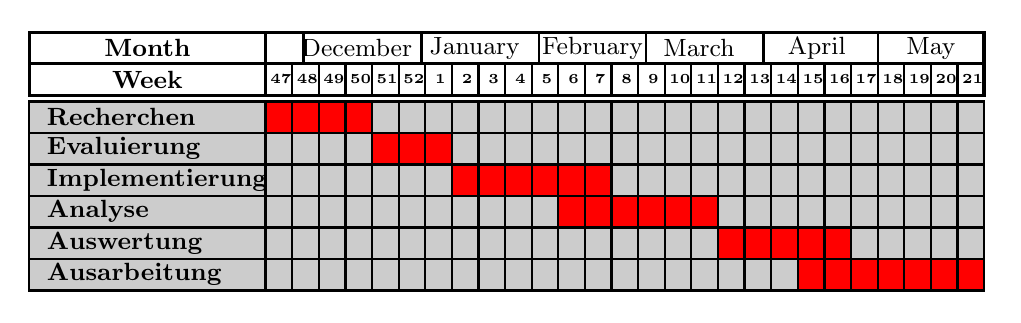
\begin{tikzpicture}
	\GanttHeader{2021-11-21}{2022-05-29}{\textwidth}
	
	
	\Task{1}{Recherchen}{0}{4}
	\Task{2}{Evaluierung}{4}{3}
	\Task{3}{Implementierung}{7}{6}
	\Task{4}{Analyse}{11}{6}
	\Task{5}{Auswertung}{17}{5}
	\Task{6}{Ausarbeitung}{20}{7}
	\end{tikzpicture}
	
	




\section{Risk Analysis}

Computation effort might not be lower than the effort for regular Matrix vector Product. 
\newline\textbf{Likelihood:} Risk is hard to determine upfront as it depends on how fast the $a_i$ decrease and on how sparse the $u_i$ and $v_i$ are. 
\newline\textbf{Mitigation:} Derive the cost and the allowed cost in an early stage of the thesis, consider Transformation in other structure.

Unable to find an appropriate algorithm 
\newline\textbf{Likelihood:} Quite likely as it is a very underdetermined problem with many parameters 
\newline\textbf{Mitigation:} use more computation-time, reduction of degrees of freedom by requiring some artificial condition (e.g. set the structure of the submatrices)

Performance will not be good 
\newline\textbf{Likelihood:} unlikely as other student work with different structures have shown that they perform quite well.
But it is unclear if it will outperform the cropped SVD
\newline\textbf{Mitigation:} difficult as it is very inherent to structure, also unlikely that it will be possible to give a definite answer that it is impossible, if the efforts fail.

\printbibliography

\end{document}
